% Just realized: b/c of anonymity, the PC can't chastise us for
% running our system on our own code -- we can't tell them that it's our code!

%Our evaluation of \projectname~leaves open several questions, which we discuss
%here.

\eat{
\noindent{\bf Aren't SDN controllers relatively simple and bug free?}
It is true that the freely available SDN applications we investigated are relatively simple. However, they
are most definitely not bug-free since, in a short period of time, we were able to demonstrate bugs in all of them. 
Production SDN controller software is far more complex than freely
available software, for a variety of reasons. Larger deployments cannot be managed with reactive microflows, and thus
require more complex proactive or hybrid strategies. As described in \S\ref{sec:overview}
fault tolerance, scale, high churn, and stringent invariants are difficult
design requirements to uphold.
SDN controllers also interact with
cloud orchestration platforms and must correctly react to concurrent changes on
their north- and southbound interfaces~\cite{netvirt}. Thus, we expect that
these production SDN control software will continue
to be under active development, and have ongoing issues with bugs for years to come. From our conversations with several SDN
controller vendors, we are aware that they all invest significant resources to troubleshooting. Several commercial players have voiced
interest in our tool as a way to improve their troubleshooting.
}

\eat{
\colin{Hopefully not necessary:}
\noindent{\bf Aren't the bugs described here trivial in nature?} Yes, the bugs we found were trivial, but that
is evidence that without better troubleshooting tools tracking down even trivial bugs is difficult.
We were particularly
surprised how quickly our tool was able to identify policy violations in the
standard routing modules of \emph{all} investigated platforms, because we assumed that the routing modules would have been well-tested
through years of use. However, these bugs remained undiagnosed because they arise from
unexpected interactions between different elements in the control plane (e.g.,
shortest path routing and topology discovery). We expect more complex bugs to
surface once we aim our tool at more complex platforms, such as those used in production settings.
}

\eat{ % No longer relevant
\noindent{\bf Are simulated failures really indistinguishable from actual
failures?} There will always be some failure modes observed in practice that are
not reproducible without adding significant complexity to the \tester. Our
approach is not particularly well-suited to model fine-grained low-level
behavior, especially on the data plane, e.g., when switches are dropping
packets due to memory or slow path constraints. Conversely, our approach excels at
investigating corner cases in distributed control plane interactions, which
are the source of many complex bugs. That said, as the system is entirely
built in software, it is in principle possible to add more fine grained
low-level behavior simulation at the cost of performance (with logical clock
speeds adjusted accordingly).  Additional experience with production systems will help
us determine how to best trade off improved simulation fidelity against degraded performance.
}

\noindent{\bf Will this approach work on all controllers?} We make limited
assumptions about the controller software in use. Three of the five platforms
we investigated were exercised with \projectname~without any modifications.
Limited changes to the controller platforms (\eg~overriding
{\tt gettimeofday()}) can increase replay accuracy further.
In general, we expect \projectname~to support controllers conforming to
OpenFlow~1.0. % out of the box.

\noindent{\bf Why do you focus on SDN?} SDN represents both an
opportunity and a challenge. In terms of a challenge,
SDN control software---both proprietary and open source---is in its infancy, which means
that bugs are pervasive.

In terms of an opportunity, SDN's architecture facilitates the implementation
of systems like~\projectname. The
interfaces between components of the system
(\eg~OpenFlow for switches~\cite{openflow} and OpenStack
Neutron for management~\cite{quantum}) are well-defined, which is
crucial for codifying functional equivalencies. % Moreover, controllers are small in number compared
% to the size of the overall network, making it easy to interpose on messages.
Moreover, the control flow of SDN control software repeatedly returns to
a quiescent state after processing inputs, which means that many inputs can be pruned.

%SDN control platforms have two properties that make
%them particularly amenable to an automated troubleshooting approach such as
%ours. First, and most importantly, SDN control software is designed to quickly
%converge to quiescence---that is, SDN controllers become idle when no policy or
%topology changes occur for a period of time.\footnote{Complex bugs may occur when
%several such processes overlay.} This means that most inputs are not relevant
%to triggering a given bug, since the system repeatedly returns to a valid
%quiescent state; often there is only one critical transition from the last
%quiescent valid configuration to the first invalid configuration. If this were
%not the case, it is not clear that the minimal causal subsequences found by our
%technique would be small, in which case our approach would not yield significant
%advantages.

Although we focus on
troubleshooting SDN control software, we believe that our general approach can
be applied to other distributed systems.
In future work we hope to validate our
technique on other such systems. % such as replicated state machines or NAS
% controllers.

\noindent{\bf Dataflow analysis.} Another avenue for future work would be to apply
dataflow
analysis~\cite{Lee:2011:TGR:1993498.1993528,tallam2007enabling}
to further prune events.
The simplest form of dataflow analysis involves
reasoning about happens-before relations: if you consider a
software-defined network as a distributed state machine,
then one can safely prune an input event if
it does not induce any messages before
the occurrence of the invalid
configuration~\cite{Lamport:1978:TCO:359545.359563}.
% since it could not have possibly affected the outcome
Unfortunately we found that pruning inputs in this way does not
significantly reduce the number of inputs, but one might go further by
analyzing the control software itself.
%code that generates messages
%to reason about which inputs have a causal linkage to the bug of interest.
% Maybe just try to apply dataflow analysis to the mock network's code, not to
% the control software code. That way we aren't language dependent.

%Along a similar vein, dataflow analysis has the potential to help address the
%problem described in~\ref{subsec:timing_heuristics} of timeouts adversely affecting replay;
%if one could infer which internal events in a subsequence are not going to
%occur, \projectname's replay scheduler would not need to timeout
%unnecessarily.

\noindent{\bf Optimizing delta debugging.} Delta debugging is agnostic to how
input sequences are split. Currently we
split by time, but it may be more effective to split events by type or by location in the network
topology.% may yield faster minimization, since bugs will often only involve a
%small number of nodes in the distributed system.

\noindent{\bf Enabling analysis of production logs.} \projectname~does
not currently support minimization of production (as opposed
to QA) logs. Production systems would need to include Lamport
clocks on each message~\cite{Lamport:1978:TCO:359545.359563} or have
sufficiently accurate clock synchronization to obtain a happens-before
relation. Inputs would also
need to need to be logged in sufficient detail for \projectname~to
replay a synthetic version. Finally, without care, a single
input event may appear multiple times in the
distributed logs. The most robust way to
avoid redundant input events would be to employ perfect failure
detectors~\cite{chandra1996unreliable}, which log a failure iff
the failure actually occurred.

\eat{ % LONG VERSION
\projectname~does not currently support minimization of production (as opposed
to QA) logs.
Here we present a sketch of how \projectname~might support production logs as input.

While we take as input a single, totally-ordered log of the events in the
distributed system, production systems maintain a log at each node.
Production systems would need to include Lamport
clocks on each message~\cite{Lamport:1978:TCO:359545.359563} or have
sufficiently accurate clock
synchronization~\cite{corbett2012spanner} to obtain a partial global ordering
consistent with the happens-before relation.\footnote{
Note that a total ordering is not needed, since it is permissible
to reorder concurrent events from
the production run so long as the happens-before relation is
maintained~\cite{Fischer:1985:IDC:3149.214121}.} Inputs would also
need to need to be logged in sufficient detail for \projectname~to
replay a synthetic version of the input that is indistinguishable (in terms
of control plane messages) from the original.

Without care, a single input event may appear multiple times in the
distributed logs. A failure of the master node, for example, could be independently
detected and logged by all other replicas. The most robust way to
avoid redundant input events would be to employ perfect failure
detectors~\cite{chandra1996unreliable}, which log a failure iff
the failure actually occurred.\footnote{Perfect failure detectors can be
implemented in partially synchronous distributed systems by explicitly killing
nodes that are suspected to be down.} % Ensuring that a single failure detector is in charge of logging node failure
% events guarantees that redundant events do not appear.
Alternatively, one
could employ root cause analysis
algorithms~\cite{yemini1996} or manual inspection to consolidate redundant
alarms.
}


%\noindent{\bf Optimizing for reproducibility, not minimality.}
%Often non-determinsm is a killer, and a slightly inflated MCS will be better than
%an MCS that very rarely is able to reproduce the bug.

%\begin{itemize}
%\item Aren't these types of bugs (e.g. failover logic) rare? Why should we
%focus on them? $\rightarrow$ msoft citation on how many man-hours it takes to debug concurrency errors
%\item What if there are causal dependencies between inputs events that we don't capture?
%\end{itemize}

% ----------------------------------------- %
%           OLD TEXT
\eat{


\noindent{\bf How big is the log? How long does this take to run?}
Assuming that it takes constant time to inject an external input, the
runtime of the algorithm is $O(n^2)$, where $n$ is the number of external inputs to
prune. If the log is too long to rerun from the beginning for
every iteration, the operator can take causally-consistent
snapshots~\cite{Chandy:1985:DSD:214451.214456} of the
live system and bootstrap the simulator from the nearest quiescent snapshot.
The length of the execution can also be `compressed' by manipulating timers in the
controllers while still maintaining happens-before dependencies. Lastly, note
that although the worst-case runtime of \simulator{} must be at least $O(n)$
(since any of the inputs may be part of the MCS), the average-case runtime of
the algorithm may be optimized by running multi-key binary search rather than
linear search.

\noindent{\bf Isn't a global log difficult to obtain?} Some failure events may appear
multiple times in the log (\eg{} replica servers detecting that a master went down),
yet we only want to replay the original event.
If it is not possible to distinguish the original
failure event from the resulting events (\eg{} in the case of a disk failure
where the original crash message is not recoverable), developers may need to
manually decipher the original event.
If the simulator is unable to reproduce the correctness violation,
the simulator may be able to `fuzz' different event
orderings in an attempt to retrigger it.

\noindent{\bf What if there are causal dependencies between inputs events?}
Developers need to know how the
distributed system {\it reacts} to external inputs. Understanding why external
inputs occurred is an orthogonal issue.
Consider a mud slide that causes (i) an network uplink to fail, which subsequently
causes (ii) a switch to overheat and crash. Our
system views (i) and (ii) as causally independent, and that's fine, since
the developer's goal is not to reason about the cause of the switch
overheating or the cause of the link failure, only how the distributed system reacted to
those events.


\colin{Discuss applicability to distributed systems besides SDN}

%\noindent{\bf How is this specific to SDN?}
%
%Yes!

\eat{
Second, we hope to gather error logs from real production deployments which
will help us populate this repository; this may require providing novel kinds
of anonymization, so that large datacenter operators would be willing to share
their problems (since they want their SDN code to work) without revealing the
details of their network.  This may require a infrastructural counterpart to
minimally-causal events; the smallest number of infrastructure components that
can reproduce the same bug.
}

\eat{
\colin{TODO: add note about not being able to tell difference between
endogenous and exogenous events, which might hide the true cause of a bug.
This is OK though, since we assume that the platform should always have a
correct option, but it doesn't take it. That is, the root cause of the crash
is not what we're interested in (software vs. hardware), it's how the platform
reacts to that crash that matters (should be robust, no matter what the
cause of the crash)}

\andi{Don't quite know what you mean by endogenous vs. exogenous}

\colin{Note that we also assume an out-of-band management network between
switches and controllers, and that the management network always provides 
connectivity. We could add the management network into our model if we want, I
suppose.}
}

\eat{ % The production environment logs this anyway? Add this point in
      % if we have space.
\noindent{\bf Aren't the proposed production logs going to be huge?}

In contrast to general record-and-replay
mechanisms, the amount of recorded state needed for
high-fidelity replay is tractable\andi{Check with our newly, well defined strong assumptions: 
we need full internal/external events. Is this tractable}. With proactive flow installation,
updates are pushed to routing tables over a relatively long time scale; periodic
FIB snapshots along with a log of link state events, control server
downtime, host mobility information, and policy-changes suffice for our purposes.
Assuming a maximum of 256K routing or ACL entries per switch~\cite{cisco7000}, and 
36 bytes per entry, each FIB will contain a maximum of 9216
kilobytes, uncompressed. A fat tree network of 27,648 hosts
includes 2,880
switches~\cite{Al-Fares:2008:SCD:1402958.1402967}.
Therefore a snapshot of the FIBs of the entire network would naively take up roughly
26 GB. Note however, that the data is likely to be compressible quite well, due to do its
structural and temporal properties. Assuming 8.5 error events per minute per
datacenter~\cite{Greenberg:2009:VSF:1592568.1592576}, 1,000,000
VM placement changes per day per datacenter~\cite{Soundararajan:2010:CBS:1899928.1899941},
and a small rate of human-specified policy changes, the log of the external inputs
should grow at a rate of \textasciitilde 750 entries per minute.
}

%To account for host mobility, assume that each server hosts 10 VMs,
%and 1\% of VMs are created, suspended, or migrated every minute. Then 10,000 host mobility events must be
%logged per minute, also a reasonable storage cost.

\eat{
\colin{Notes from Rean Griffith:
\begin{itemize}
\item total vms in a typical datacenter: 1000
\item migration frequency (migrations/minute): 20 per hour
\item VM spin ups/downs: 150 power ons per hour (see our OSR 2010 paper for
power off estimates)
\item Do we log VM migrations and how does that log grow (I wasn't able to
get any estimates on log-growth data)
\end{itemize}

We had an OSR 2010 paper that provided numbers scaled by the number of
VMs in an installation:
Challenges in building scalable virtualized datacenter management
(http://dl.acm.org/citation.cfm?id=1899941)
}
}

%As a point of reference, border routers' working RIB size is
%$\textasciitilde$130MB~\cite{Karpilovsky:2006:UFR:1368436.1368439}.
\eat{

TODO: Replace this analysis.
It stinks. PORTLAND is not the right way to evaluate this due to the lacking number of rules.

\noindent{\bf Correspondence Checking Runtime.} 
Computing the propagation
graph for correspondence checking is equivalent to enumerating
all possible paths in the network, which scales with the diameter
of the network and the number of routing entries per switch.
The propagation graph for each host can be
computed in parallel however, so the computation is bottlenecked by the serial runtime
of computing a single host's propagation graph.

We show the serial runtime of correspondence checking in
Figure~\ref{fig:hsa_runtime}. For this analysis we generated fat tree topologies
between 2 and 48 pods wide, with pre-installed PORTLAND~\cite{NiranjanMysore:2009:PSF:1592568.1592575}
routing tables in each switch. Each data point is the minimum of three
runs on a single Intel Xeon 2.80GHz core. Note that the number of PORTLAND routing entries per switch scales with the number
of pods in the fat-tree. We excluded the time to convert
flow tables to HSA transfer functions, since transfer functions can be maintained
offline.

As the figure depicts, even for large networks
(27,648 hosts) the serial runtime of correspondence checking is reasonable for
interactive use. The number of serial tasks to be executed
is the number of hosts in the network squared, disregarding ECMP load balancing.

\begin{figure}[t]
    %\hspace{-10pt}
    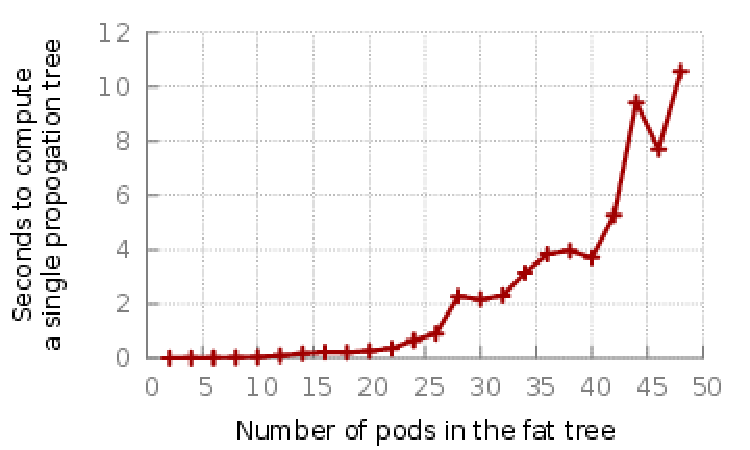
\includegraphics[width=3.25in]{../graphs/hsa_overhead_graph/graph.pdf}
    \caption[]{\label{fig:hsa_runtime} Serial runtime of correspondence
    checking on PORTLAND fat tree networks. Each datapoint consists of
    $x^3/4$ hosts and $5x^2/4$ switches (\eg{} 48 pods means 27,468 hosts
    attached to 2,880 switches)}
\end{figure}
}

\eat{ This evaluation stinks. Be gone!

\noindent{\bf Simulator Scalability.} As our approach depends on the frequently
repeating simulations, we now evaluate the setup time incurred by the simulator
system when handling large network topologies. For this experiment, shown in
Figure~\ref{fig:scalability}, we generate fat tree topologies between 2 and 48
pods wide, where all switches in the network connected to a single controller.
The controller sends each switch an OpenFlow $FLOW\_MOD$ and subsequent
$BARRIER\_REQUEST$ message, and waits for the corresponding $BARRIER\_REPLY$. We
then measure the time to between the first $FLOW\_MOD$ sent and the last
$BARRIER\_REPLY$ received. As expected, the runtime was roughly linear with the
number of switches in the network. The figure also shows that the processing
time for large networks (5 seconds per simulator round) was well within the
bounds for interactive use.

\begin{figure}[t]
    %\hspace{-10pt}
    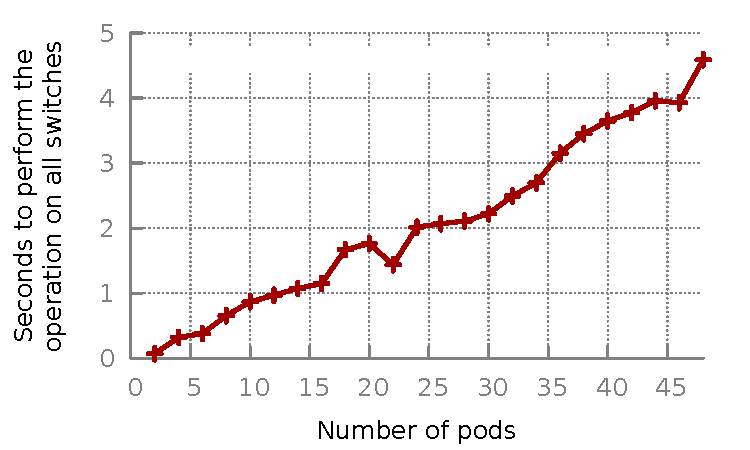
\includegraphics[width=3.25in]{../graphs/scalability_graph/scale.pdf}
    \caption[]{\label{fig:scalability} Time to send and process messages
    between controller and simulated switches. Each datapoint consists of
    $x^3/4$ hosts and $5x^2/4$ switches (\eg{} 48 pods means 27,468 hosts
    attached to 2,880 switches)}
\end{figure}

We also tested the extreme limits of the simulator's scalability, pushing up
the number of switches until something broke. We encountered what appears to be
a limitation of the Linux TCP/IP stack: TCP connection attempts began failing
beyond 26,680 sockets. Note that 26,680 switches is an order-of-magnitude larger than
the today's biggest networks.
}

}
